% https://plantuml.com/de/timing-diagram

\textcolor{red}{mit MEASUREMENT Flag kompiliert um zu testen}

% Netzwerklatenz & andere Latenzen!!!
% Implementierung: Roboter wählt seine eigene Bahn

% da ein Delay von < 50 ms aufgrund der Gestenerkennung nicht eingehalten werden kann muss die Berechnung des neuronalen Netzwerks der Gestenerkennung noch schneller werden bzw. auf speziell darauf ausgelegter Hardware (FPGA) ausgeführt werden

% Die Orientierung ist meisten nicht so wichtig. Daher kann diese in einigen bestimmten Fällen auf ein paar Grad genau getestet werden mittels optischen Test bzw. im Simulator

% Wie lange benötige ich für das Teachen mittels Gesten? Ist es ein vertretbarer Aufwand? Was ist ein vertretbarer Aufwand?

% Speziell das Echtzeitverhalten ist eher subjektiv zu betrachten, da jeder die Latenz zwischen Ein- und Ausgabe ein klein wenig anders wahrnimmt.

% Hierfür wurde darauf geeinigt, dass die Bewegungsabläufe des Roboters auch nachträglich nachbearbeitet werden können.

%Die Tests erfolgen in einem virtuellen Raum, in welchem die exakten Positionen bereits vordefiniert sind.
% Die ermittelten Positionen können dann mit den exakten Positionen verglichen werden und wiederum Kennwerte, wie z.B. der Mittelwert, Standardabweichung, Varianz ermittelt werden.

% Wünschenswert, die Bewegungen können jedoch aber im nachhinein auch nachträglich nachbearbeitet werden. Wenige mm wären ideal, aber wenige cm würden auch genügen.

% Bewegen durch Gesten in beliebigen Koordinatensystemen mit unterschiedlichen Orientierungen

% Herkömmliche Eingabegeräte (z.B. ein Teach Pendant) vs. ein NUI-System (z.B. Azure Kinect mit Tiefensensor zur Erkennung von Gesten); Vergleich mit bisherigen Teach-Lösungen, wie z.B. einem Teachpendant; Die Probanden sollten fachkundig sein und wenn möglich bereits Vorerfahrung mit Möglichkeiten zum Teachen von Robotern haben. -> ist schwer möglich ohne die entsprechende Hardware

% ------------

% Azure Kinect: Belichtungszeit: 1,6 ms bis zu 20,3 ms (https://docs.microsoft.com/en-us/azure/kinect-dk/hardware-specification) -> TODO: Passive IR einschalten?
% Realsens: Belichtungszeit: 900 ns (https://www.imveurope.com/press-releases/intel-realsense-lidar-depth-camera-l515) (https://softei.com/framos-claims-hi-res-intel-realsense-lidar-depth-camera-is-worlds-smallest/) (https://venturebeat.com/2019/12/11/intels-new-realsense-camera-packs-a-lidar-sensor-for-enhanced-depth-perception/) -> Distanz?
% https://www.intelrealsense.com/compare-depth-cameras/
% https://www.intelrealsense.com/depth-camera-d435/

% https://docs.microsoft.com/en-us/windows/mixed-reality/ISSCC-2018



%----------------

% https://feedback.azure.com/forums/920053-azure-kinect-dk/suggestions/38129473-body-tracking-without-cudnn
% https://feedback.azure.com/forums/920053-azure-kinect-dk/suggestions/39945454-legacy-body-tracking-like-kinect-v2
% https://github.com/microsoft/Azure-Kinect-Sensor-SDK/issues/1080



%-----------\\
% konkrete Aussage zur Performanz, Stabilität, Modularität, Hohe Skalierbarkeit,
% Erweiterbarkeit

% Erfahrungen

% Mögliche Prognosen

% Limitierungen

% Entwicklungswerkzeuge


% --------------\\

% Andere Vergleiche in der Literatur


\textcolor{red}{TODO:\\
Was wird in diesem Kapitel beschrieben?\\
Visualisierung:\\
* Diagramme\\
* Mittelwert, Standardabweichung, Varianz, ...
}

% weiche Echtzeitfähigkeit
% Durchsatz, Latenzen, ...

% Die Gestensteuerung des WidowX 200, welches auf dem für diese Arbeit erstellten Roboter-Gesten-Framework basiert und als Basis für andere gestengesteuerte Roboter dienen kann, wird auf die Ergonomie, Echtzeitfähigkeit, Genauigkeit der Gestenerkennung und Genauigkeit der Zielpositionen hin überprüft. Zudem wird ROS 1 auf die Netzwerklatenz hin überprüft um darauf basierend eine Einschätzung zu gegeben ob sich ROS 1 für echtzeitfähige Systeme eignet.


% Durchsatz, Latenzen, ...\\
% Zeit zur Erkennung von Gesten (Azure Kinect Body Tracking SDK: beinhaltet Latenz von Aussenden des Infrarot-Lichtimpuls bis zum Empfang zur Absorption des Lichtimpuls, durch Belichtungszeit bis hin zur Latenz über das \quoteMark{USB 2.0}-Kabel)?\\



\section{Latenz der Gestenerkennung}
\textcolor{red}{Azure Kinect im CPU-Modus anstatt mit Grafikkartenbeschleunigung, weil keine Nvidia Grafikkarte vorhanden war und der kleinste gemeinsame Nenner gewählt wird}

Die Datei \quoteMark{gestures\_recognition\_measurement.txt} ist auf der CD/ISO im Verzeichnis \quoteMark{Ergebnisse/} zu finden.

\begin{figure}[htb]
	\centering
	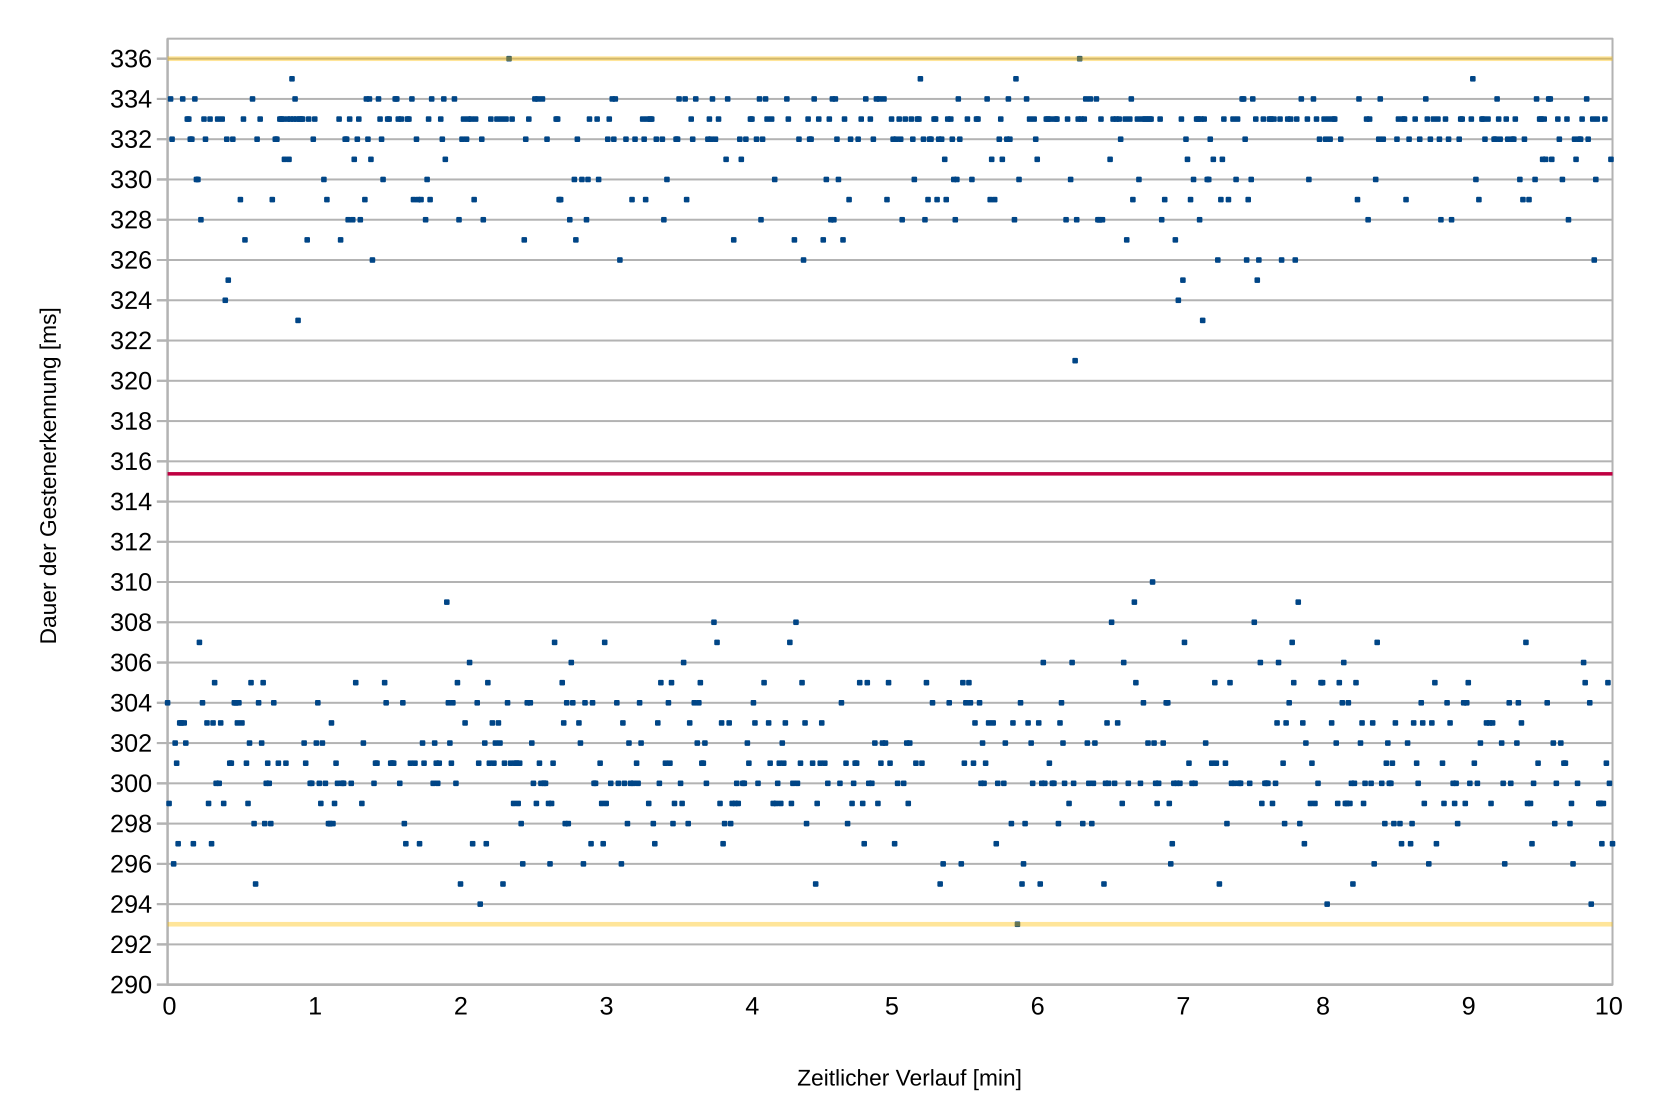
\includegraphics[width=1.0\textwidth]{images/ergebnisse/dauer_der_gestenerkennung_verlauf}
	\caption[Zeitlicher Verlauf der Gestenerkennung der Azure Kinect]{Zeitlicher Verlauf der Gestenerkennung der Azure Kinect\\Quelle: Eigene Ausarbeitung}
	\label{fig:sched_deadline}
\end{figure}
\FloatBarrier


\section{Latenz der Übertragung mit und ohne ROS-Anbindung}
\textcolor{red}{TODO:\\
Praxistest mit zusätzlicher Gestenerkennung oder ohne?\\
WidowX 200\\
Verschiedene Netzwerkkonstellationen simulieren? % aus dem Sicherheitsaspekt sollte für ROS 1 ein eigens für den Roboter abgeschottenes Netzwerk verwendet -> dadurch meisten weniger Latenzen, weil weniger über ROS übertragen wird?
% http://wiki.ros.org/Topics
% Topic statistics
}

% für ROS: ein Testnetzwerk aufbauen unterschiedliche Latenzen testen
% Best Case: keine Latenzen
% Worst Case: Übertragen von größeren Datenmengen über ROS (z.B. Kamerabilder, …)

% vom Übertragen des Befehls an die Steuerungseinheit bis der Roboter die Bewegung durchführt
%vom Übertragen des Befehls über TCP/IP bis zur Steuerungseinheit
%vom Durchführen der Geste bis zum erfolgreichen Erkennen von unterschiedlichen Gesten. Unterschiedliche Gesten können mitunter z.T. mehr oder weniger Zeit beanspruchen je nach Komplexität der Geste.


\section{Genauigkeit der Ziele}
\textcolor{red}{TODO}

%Im Vergleich zu einer anderen Eingabemethode%\\
%PS3-Controller: https://www.trossenrobotics.com/widowx-200-robot-arm.aspx

% Wie genau kommt man ans gewünschte Ziel? (Einheit: mm)
% Wie viele Korrekturen braucht ein Proband um am nächsten ans gewünschte Ziel zu kommen?

% In einer realen Umgebung nur mit Ungenauigkeiten messbar
%In einer Simulationsumgebung (z.B. Gazebo) kann die Distanz genau und automatisiert gemessen werden
%Visualisierung:
%  *Diagramme
%  *    Mittelwert, die Standardabweichung, Varianz, ...


\section{Genauigkeit der Gestenerkennung}
% Wie viele Versuche benötigt ein Proband bis seine Gesten erkannt werden?

\section{Ergonomie \& User Experience}
% Verbessert dieser Ansatz die Ergonomie des Teachen in eine positive Richtung?
% Ist es angenehmer diese NUI-Methode zu verwenden als ein herkömmliches Teach Pendant?
% Kann ich über eine längere Zeitspanne, wie z.B. 30 Minuten, einen Roboter teachen?
% Wie schnell bin ich erschöpft im Gegensatz zu einem herkömmlichen Teach Pendant?
% Wie schnell erlernt man die Gesten?
% Wie einprägsam sind die Gesten?
% Sind die Gesten gut geeignet um einen Roboter zu steuern oder sind diese zu schwammig oder zu ähnlich und werden daher auch oft verwechselt?
%   * Können diese im besten Fall nur schwer unbeabsichtigt durchgeführt werden und fälschlicherweise nicht z.B. als kulturelle Geste erkannt werden?
%   * Gibt es wenige Überschneidungen mit bereits definierten Gesten, sodass diese nicht unbeabsichtigt durchgeführt werden können?
%   * Sind diese leicht anzuwenden, sodass das System die Geste im besten Fall beim ersten Mal erkennt?

% Erkennungsrate der Gestenerkennung

\textcolor{red}{TODO:\\
Wie gut ist das System einsetzbar? UX\\
Bewertung der Ergonomie über längere Zeitdauer (sehr subjektiv, jedoch aber versuchen die Ergebnisse auf die Allgemeinheit zu bezienen)\\
Während dem Teachen bewegt man sich oft um zu sehen ob der Endeffektor an der richtigen Stelle ist. Mit einer fest angebrachten Azure Kinect ist es daher schwer den eigenen Blickwinkel zu ändern\\
reflexartige und unbeabsichtigte Bewegungen\\
Beim Teachen steht man normalerweise um den Roboter ordnungsgemäß und vollständig sehen zu können
% siehe 3.4.3 Auswahl anhand der Ergonomie
}

% muss nicht auf die Körpergröße eingestellt werden, da der Field of View sehr groß ist

% Kann ich über eine längere Zeitspanne, wie z.B. 30 Minuten, einen Roboter teachen? Wie schnell bin ich erschöpft im Gegensatz zu einem herkömmlichen Teachpendant? Wie schnell lernt man die Gesten? Sind die Gesten gut geeignet um einen Roboter zu steuern oder sind diese zu schwammig oder zu ähnlich und werden daher auch oft verwechselt?
